\documentclass[UTF8]{ctexart}
\usepackage{hyperref}
\usepackage{abstract}
\usepackage[margin=1in]{geometry}
\usepackage{graphicx}
\usepackage{gensymb}
\usepackage{float}
\usepackage{amsmath}
\usepackage{multirow}
\begin{document}

\title{第三次仿真实验报告}
\author{2019012137  工物90  张鸿琳}
\maketitle

\tableofcontents
\newpage
\section{设计正弦波发生器}
\subsection{文氏(Wien)电桥电路}
文氏电桥电路如下图:
\begin{figure}[H]
\centering
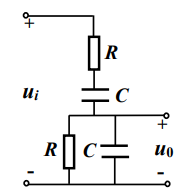
\includegraphics[width=0.2\textwidth]{A.png}
\caption{文氏电桥电路}
\end{figure}

在仿真软件中搭建的仿真电路图如下:
\begin{figure}[H]
\centering
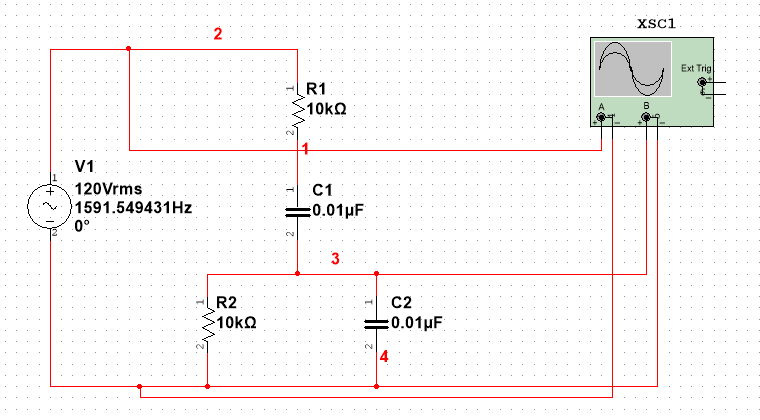
\includegraphics[width=0.95\textwidth]{C.png}
\caption{文氏电桥仿真电路图}
\end{figure}

那么$u_i$与$u_0$之间存在关系,$u_0=\frac{Z_2}{Z_1+Z_2}u_i$,其中$Z_1$为电阻R与电容C串联后的阻抗,$Z_2$为电阻R与电容C并联后的阻抗,代入已知数据化简后得到如下关系:

\begin{equation}
u_0=\frac{1}{j\omega CR+3+\frac{1}{j\omega CR}}u_i
\end{equation}

故而若要使$u_i$与$u_0$同相,则要消去虚数项,进而得到应有$R\omega C=1$,此时频率为$f=\frac{\omega}{2\pi}=\frac{1}{2\pi RC}\approx1591.549431$ Hz,且输出电压与输入电压有效值的比值为$\frac{U_0}{U_i}=\frac{1}{3}$。在仿真软件中代入此结果,得到的示波器图像(CHA对应输入电压,CHB对应输出电压)如下:
\begin{figure}[H]
\centering

\includegraphics[width=0.95\textwidth]{B.png}
\caption{$f=1591.549431$ Hz时,示波器图像}
\end{figure}

由示波器图像可以看出,输入与输出电压确实在该频率下为同相的,且电压峰值之比(等于有效电压之比)为1:3。
\subsection{设计一个放大倍数为3的放大器}
放大倍数为3的信号放大器电路原理图如下:
\begin{figure}[H]
\centering
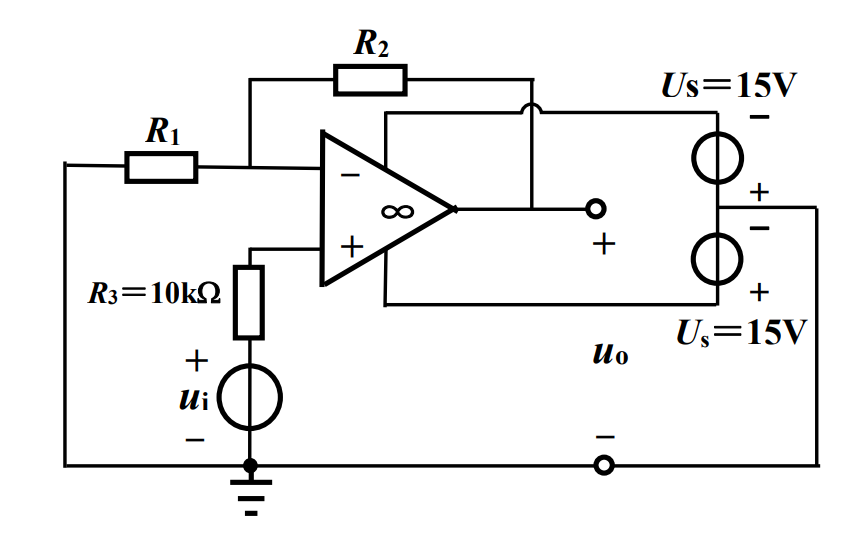
\includegraphics[width=0.65\textwidth]{D.png}
\caption{放大倍数为3的信号放大器电路原理图}
\end{figure}

为了使输出电压$u_0$为输入电压$u_i$的三倍,显然应调节$R_1$与$R_2$的阻值大小,由虚短可得,$R_1$右端电压为$u_i$,再由虚短可得,流经$R_1$与$R_2$的电流大小一样,故而有$\frac{u_i}{R_1}=\frac{u_0-u_i}{R_2}$,化简,得
\begin{equation}
u_0=\frac{R_1+R_2}{R_1}u_i
\end{equation}

所以有$R_2=2R_1$,同时为了减小偏置电流对运放的影响,需满足$R_1//R_2=R_3$,由此求得$R_1=15k\Omega$,$R_2=30k\Omega$。

仿真电路如下图:
\begin{figure}[H]
\centering
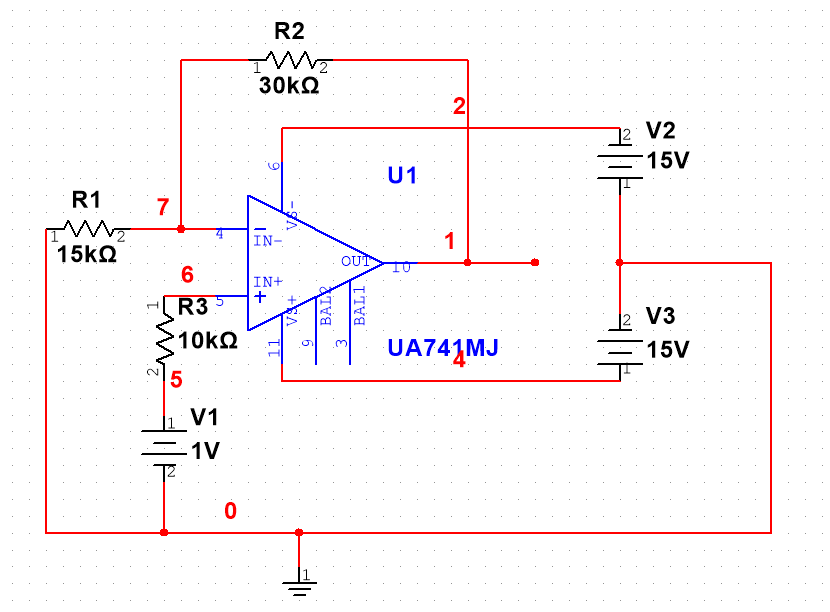
\includegraphics[width=0.85\textwidth]{E.png}
\caption{放大倍数为3的信号放大器仿真电路图}
\end{figure}

为了验证是否将输入信号放大3倍(保证运放工作在线性区),令$u_i=1V$,得到示波器图像(CHA为输入信号,CHB为输出信号)如下:
\begin{figure}[H]
\centering
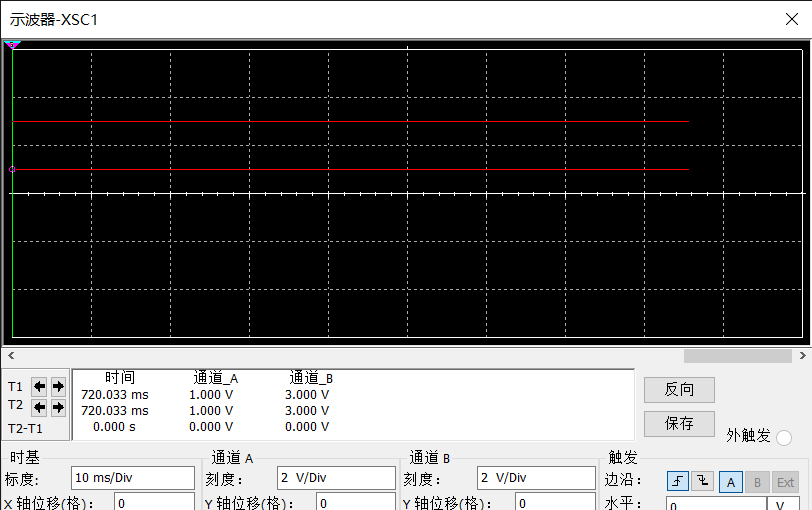
\includegraphics[width=0.85\textwidth]{F.png}
\caption{放大倍数为3的信号放大器仿真电路示波器图像}
\end{figure}


可见,该电路实现了将信号放大三倍的效果。
\subsection{由文桥电路和三倍同相比例放大器组成一个正弦波发生器}
正弦波发生器电路原理图如下:
\begin{figure}[H]
\centering
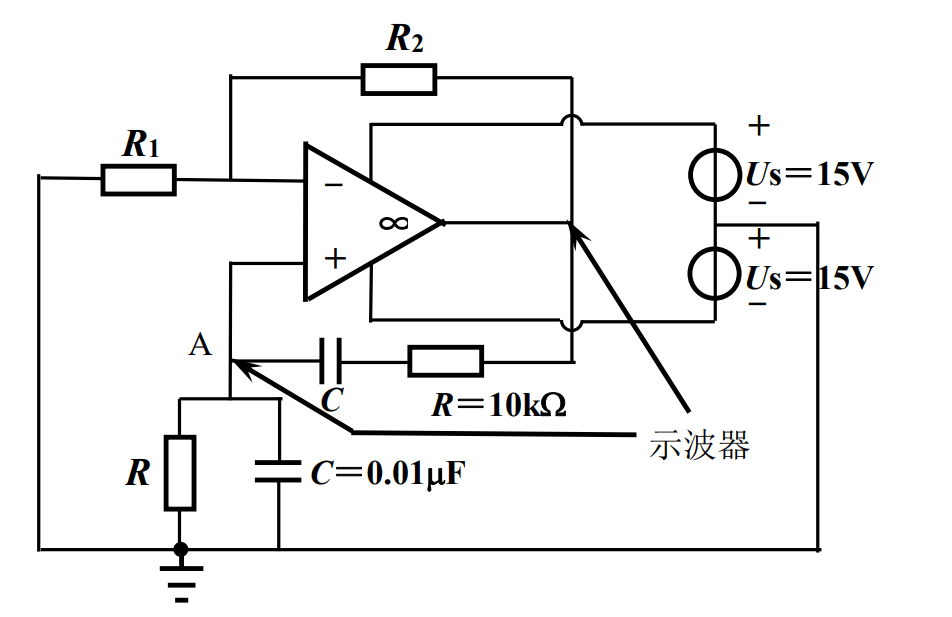
\includegraphics[width=0.75\textwidth]{G.png}
\caption{正弦波发生器电路原理图电路原理图}
\end{figure}

\textbf{首先分析为什么要采用放大倍数为3的同相比例放大器:}由电路原理图以及之前同相比例放大器的分析,可知$u_0$等于A处电压的三倍,而A处电压相当于文氏电桥电路的输出,$u_0$相当于文氏电桥电路的输入,由于放大器的输入与输出是同相的,所以可知稳定时,文氏电桥电路也必定是达到了输入与同相的稳定状态,先局部分析文氏电桥电路,有$3u_A=u_0$,再局部分析同相比例放大器,设放大倍数为$x$,则有$xu_A=u_0$,若$x\neq3$,那么就会出现矛盾,也就不存在能够稳定输出的正弦波了,所以放大倍数必须为3。

正弦波发生器仿真电路图如下:
\begin{figure}[H]
\centering
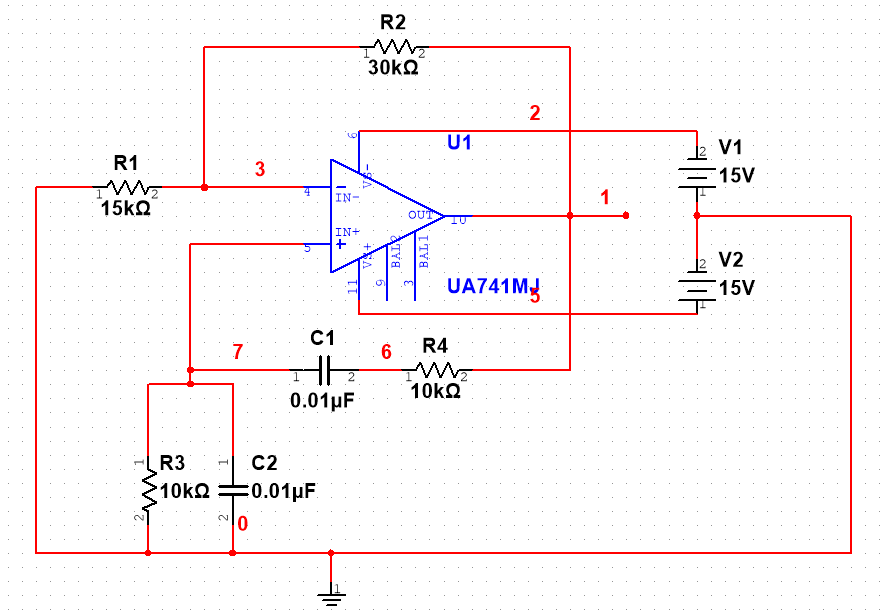
\includegraphics[width=0.95\textwidth]{H.png}
\caption{正弦波发生器电路原理图仿真图}
\end{figure}

示波器在接入原理图中的两个点位后,其显示波形如下:
\begin{figure}[H]
\centering
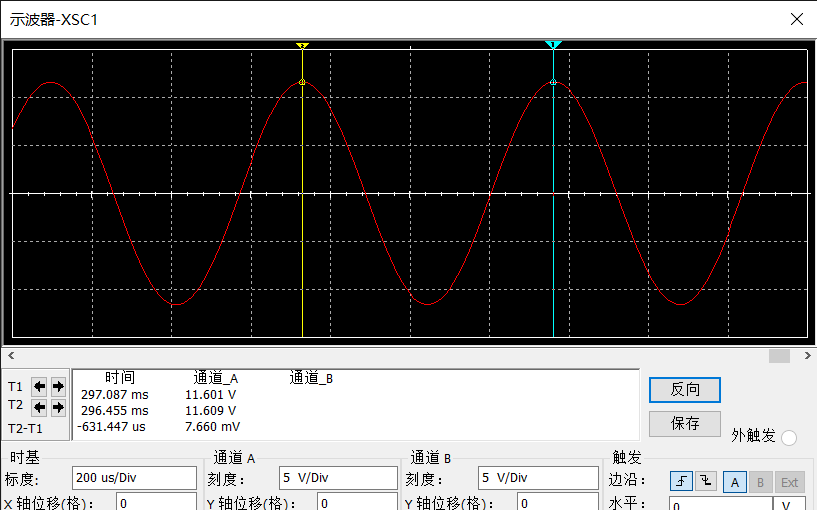
\includegraphics[width=0.85\textwidth]{I.png}
\caption{正弦波发生器电路的示波器波形}
\end{figure}

由波形图可看出,其周期约为0.632ms,电压峰值约为11.601V。

若要获得二倍频率的正弦波,则需要调节文氏电桥电路的$R$与$C$的值,由第一部分的分析,可知,只要$RC$的值为原来的$\frac{1}{2}$,那么稳定时频率就为原来的两倍,不妨令$R=5k\Omega$,此时得到的示波器波形如下:
\begin{figure}[H]
\centering
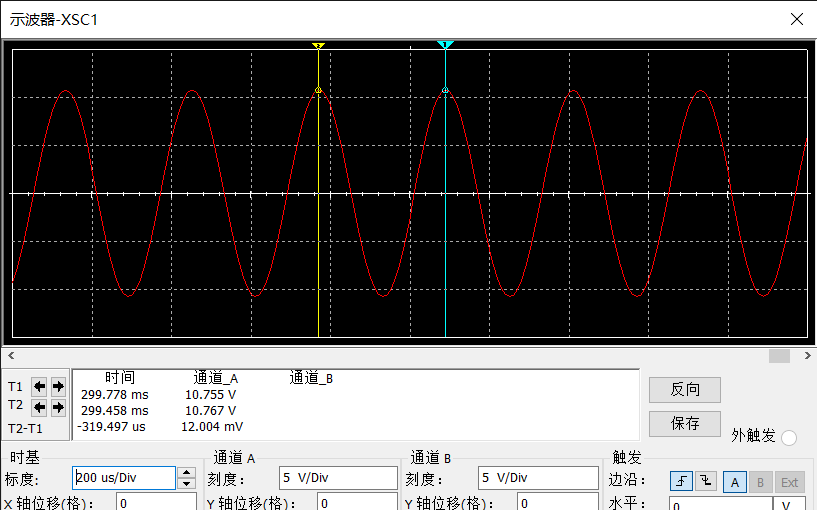
\includegraphics[width=0.85\textwidth]{J.png}
\caption{将R阻值大小变为原来一半后,正弦波发生器电路的示波器波形}
\end{figure}

由波形图,可得出此时周期约为0.320ms,电压峰值约为10.755V,周期确实变为了原来的一半,即频率加倍。
\section{设计并验证电容倍增器}
\subsection{电容倍增器电路原理图及其原理分析}
电容倍增器电路原理图如下:
\begin{figure}[H]
\centering
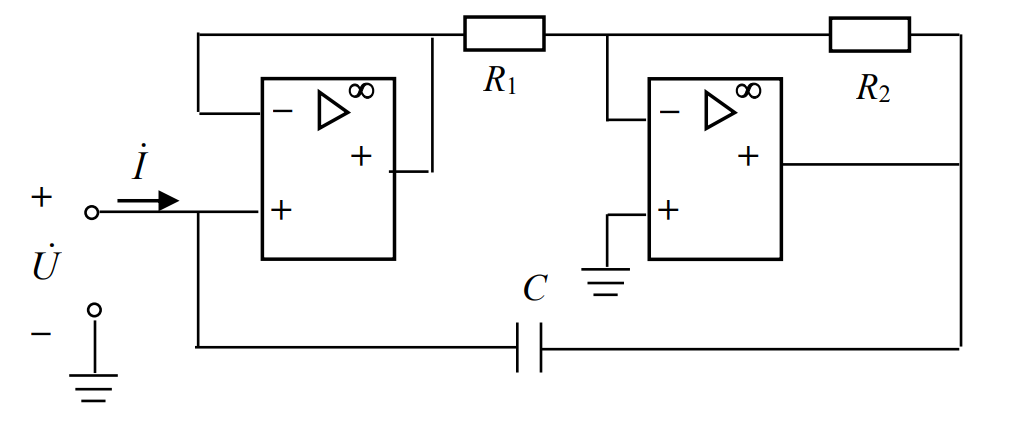
\includegraphics[width=0.85\textwidth]{K.png}
\caption{电容倍增器电路原理图}
\end{figure}

\textbf{分析其如何实现电容倍增效果:}设输入电压为$u$,电容器C左侧电势为$u_1$,右侧电势为$u_2$,由于两个运放都是负反馈,所以由虚短得,$R_1$两端电压为$0-u=-u$,$R_2$两端电压为$u_2-0=u_2$,再由虚断得,$\frac{u_2}{R_2}=-\frac{u}{R_1}$,所以有$u_2=-\frac{R_2}{R_1}u$,对于电容C则有$u_1=u$,$C\frac{d(u-u_2)}{dt}=i=\frac{C(R_1+R_2)}{R_1}\frac{du}{dt}$,所以等效电容变为$C'=\frac{(R_1+R_2)}{R_1}C$,也就是实现了电容倍增效果。
\subsection{仿真电路及其结果}
令$C$=10nF,若要利用电容倍增器使其电容变为$C'=0.11\mu$F,则由上面的分析,可知只需令$R_2=10R_1$即可,仿真电路如下:
\begin{figure}[H]
\centering
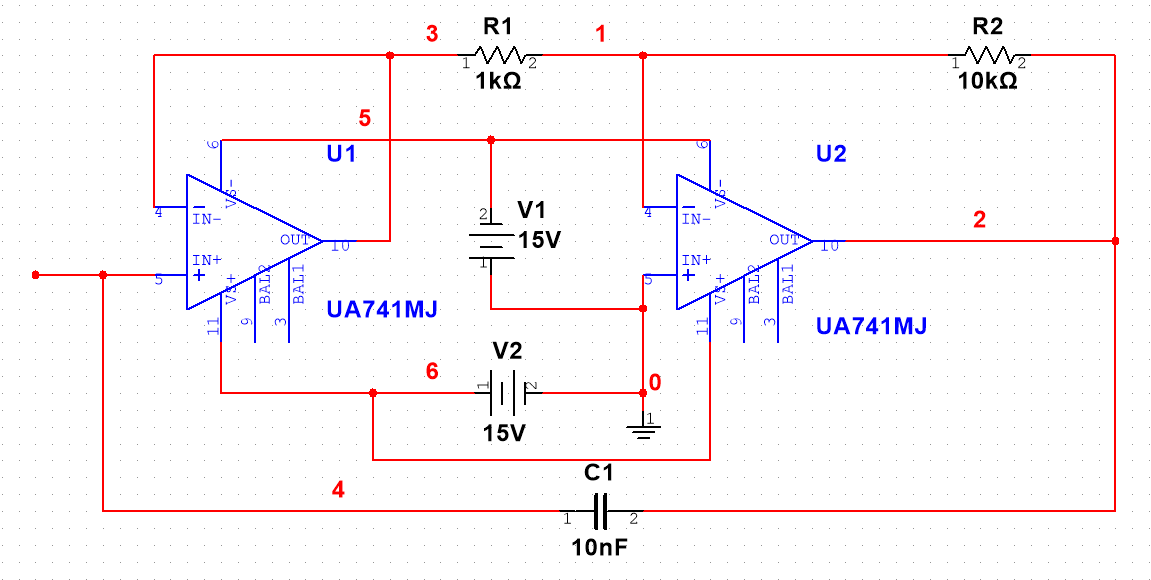
\includegraphics[width=0.95\textwidth]{L.png}
\caption{电容倍增器仿真电路图}
\end{figure}

仿真电路的示波器图像(CHA所测为输入电压,CHB对应输入电流(每1V电压对应1mA电流))如下:
\begin{figure}[H]
\centering
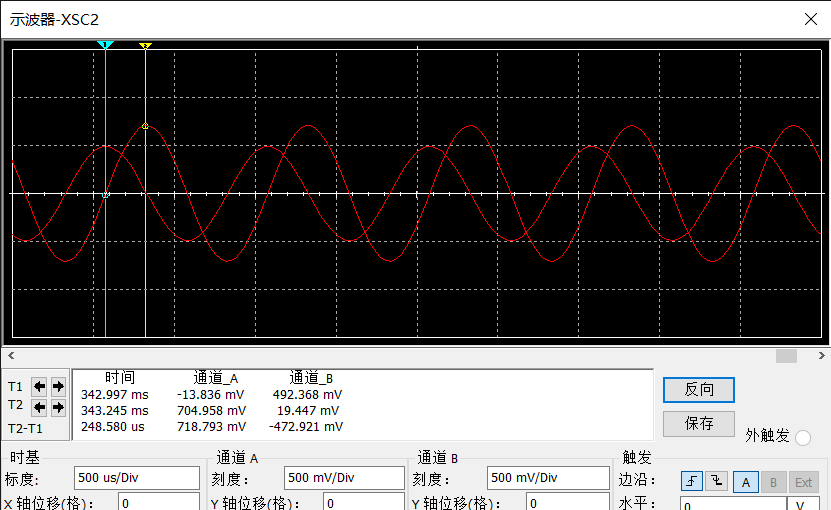
\includegraphics[width=0.85\textwidth]{M.png}
\caption{电容倍增器仿真电路的示波器波形}
\end{figure}

由图可看出电压与电流相位差为$\frac{\pi}{2}$,同时应有电流与电压峰值之比为$\frac{I}{U}=\omega C=2\pi\times1000\times0.11\times10^{-6}\approx6.9115\times10^{-4}$S,而由图中数据,二者峰值之比为$\frac{I}{U}\approx\frac{492.368}{704.958\times1000}\approx6.9844\times10^{-4}$S,与理论结果符合地比较好,该电路产生了电容倍增的效果。
\begin{thebibliography}{123456} 
\bibitem{ref1} 无
\end{thebibliography}


\end{document}
